\documentclass{article}
% Tamaño página
\usepackage[paperheight=27cm,paperwidth=21cm,textwidth=17cm ,textheight=23cm]{geometry}
% Librería lorem ipsum?
\usepackage{lipsum}
\usepackage{fancyhdr}
\usepackage{hyperref}
\usepackage{graphicx}
\graphicspath{{images/}}
\hypersetup{
    colorlinks=true,
    linkcolor=blue,
    filecolor=magenta,      
    urlcolor=cyan,
    pdftitle={Introducción a Packet Tracer - Mariano Campos},
    pdfpagemode=FullScreen,
    }

\title{\bfseries \huge Introducción a Packet Tracer \normalsize{\linebreak\\Redes de computadoras I \\Prof.: Alejandro Rodriguez Costello}}
\author{\\\\\\\\\\\\Campos, Mariano Andrés \\ {\small visual.design.90@gmail.com}}
\date{\small 21 de Agosto 2024}

\begin{document}
    \maketitle
    \newpage

    \section{Cisco Packet Tracer - Introducción}
        \subsection{¿Qué es?}
        Cisco Packet Tracer es una de las herramientas más importantes y valiosas para estudiar redes. Es un simulador de redes diseñado por Cisco que se puede descargar del siguiente \href{https://skillsforall.com/resources/lab-downloads?courseLang=en-US}{link}.

        \subsection{Herramientas básicas}
        Provee herramientas para trabajar y, entre las muchas acciones, realizar las siguientes actividades:
        \begin{itemize}
            \item Agregar dispositivos y conectarlos mediante cable o conexiones inhalámbricas.
            \item Seleccionar, borrar, inspeccionar y agrupar componentes en tu red.
            \item Gestionar tu propia red, determinando las configuraciones necesarias para cada dispositivo, es decir, tipos de conexiones, direcciones de ip, puertas de enlace, etc.
        \end{itemize}
        Permite crear redes y visualizar su forma de trabajo, las tecnologías y protocolos incorporados. Dentro de los principales menúes, en la esquina inferior izquierda encontramos el menú de dispositivos disponibles para trabajar.\linebreak

        \begin{center}
            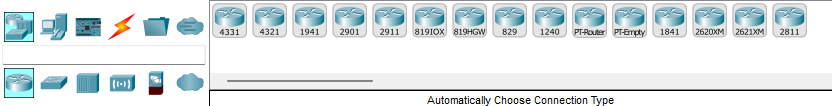
\includegraphics[width=0.65\linewidth]{img_1} 
            \linebreak
            \small {\bfseries Figura 1}: Imagen del menú de dispositivos, componentes y conexiones disponibles (entre otros).
        \end{center}

    \section{Modos de operación}
    El programa provee dos modos de operación:
    \begin{itemize}
        \item {\bfseries Modo en tiempo real}: donde la red desplegada corre constantemente, independientemente de si se está trabajando sobre la red o no. Las estadísticas de la red se muestran en tiempo real.
        \begin{center}
            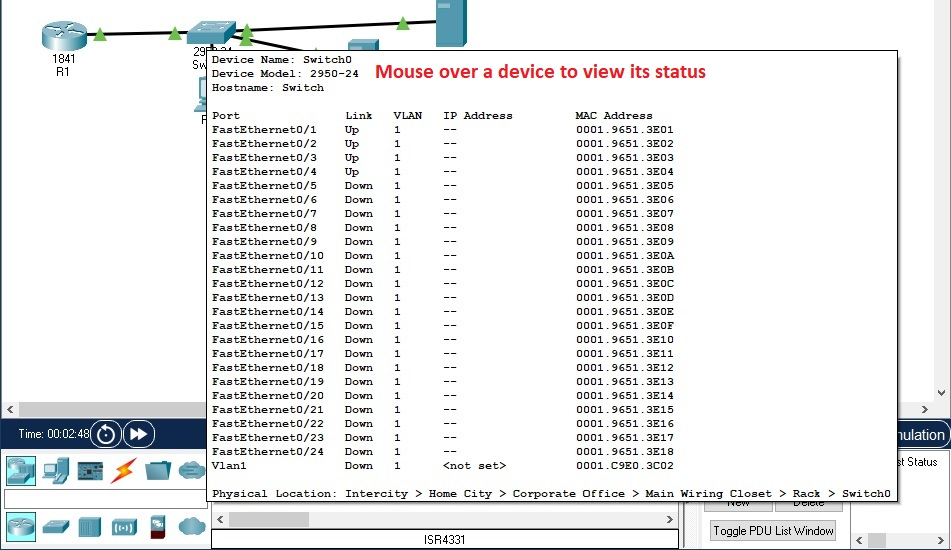
\includegraphics[width=0.85\linewidth]{img_3} 
            \linebreak
            \small {\bfseries Figura 2}: Estado en tiempo real de un Switch.
        \end{center} \pagebreak
        \item {\bfseries Modo simulación}: permite observar los caminos que recorren los paquetes e insperccionarlos, mostrando la distribución de los mismos por la red a una velocidad reducida.
        \begin{center}
            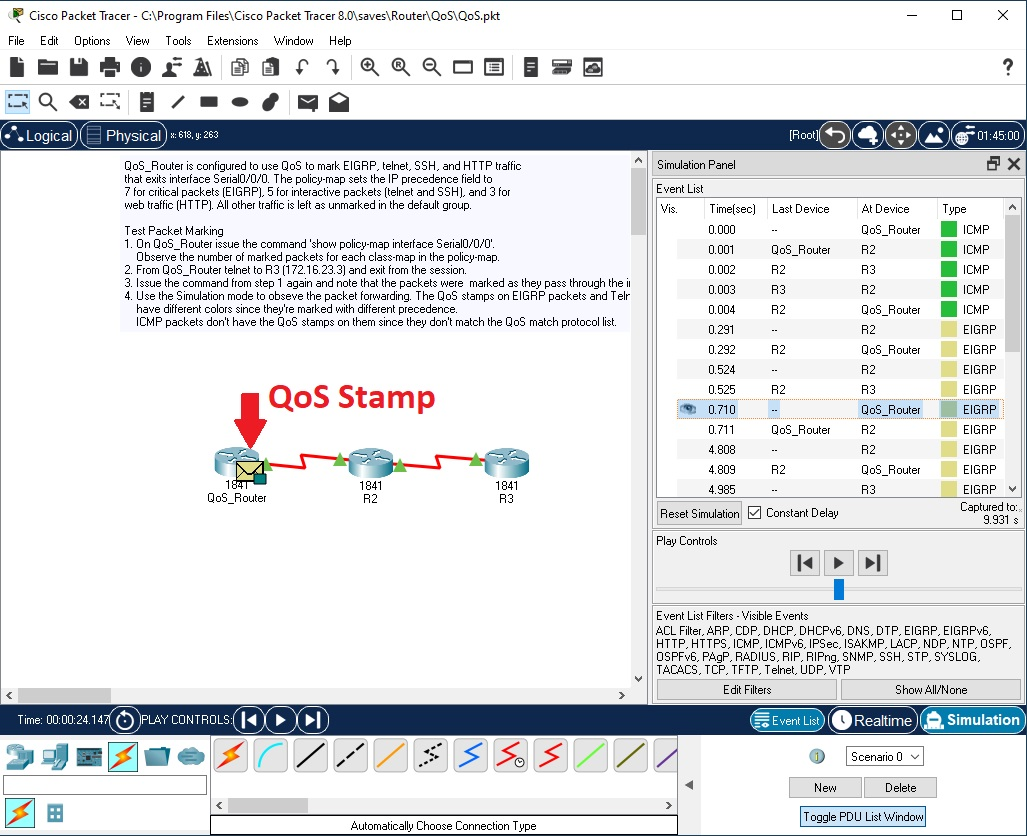
\includegraphics[width=0.85\linewidth]{img_4} 
            \linebreak
            \small {\bfseries Figura 3}: Paquete viajando a través de la red.
        \end{center}
    \end{itemize}
    Adicionalmente existen dos modos para crear los diagramas de red:
    \begin{itemize}
        \item {\bfseries Modo lógico}: permite crear un diagrama lógico de una red.
        \item {\bfseries Modo físico}: permite crear un diagrama físico teniendo en cuenta factores como distancias, disposición de las oficinas, etc. Permite crear una red más realista teniendo en cuenta las características mencionadas.
    \end{itemize}

    \section{Dispositivos finales}
    Los dispositivos finales son dispositivos fuente y destino, encargados de enviar información a una red. Estos dispositivos se diferencian unos de otros mediante una dirección. Cuando un dispositivo inicia una comunicación con otro, utiliza la dirección del destino de donde debería llegar la transmisión del mensaje. Podemos hacer referencia a los siguientes dispositivos:
    \begin{itemize}
        \item Computadora (escritorio, notebook, etc)
        \item Impresoras
        \item TV Smart
        \item Dispositivos VoIP
    \end{itemize}

    \begin{center}
        
\includegraphics[width=0.65\linewidth]{img_2} 
        \linebreak
        \small {\bfseries Figura 4}: Dispositivos finales disponibles en Packet Tracer.
    \end{center}

    \section{Dispositivos de red}
    Son dispositivos que permiten la comunicación entre el hardware de red de dispositivos como computadoras.
    \begin{itemize}
        \item {\bfseries Repetidor}: opera en la capa física, amplificando señales de una red.
        \item {\bfseries Hub}: es equivalente a un repetidor multipuerto. Conecta diferentes ramas de una red. 
        \item {\bfseries Switch}: es un repetidor multipuerto que filtra el contenido mediante una dirección MAC y tiene un buffer que permite prevenir errores antes del envío de información.
        \item {\bfseries Router}: es un dispositivo que enruta paquetes de información basados en su dirección IP. Normalmente conectan redes LAN y WAN.
    \end{itemize}
    En la vista física, los dispositivos tienen módulos que se pueden intercambiar o añadir para realizar configuraciones que suplan las necesidades del trabajo a realizar.\linebreak
    Existen muchos módulos de expansión, por ejemplo, para routers algunos de los que podemos encontrar son:
    \begin{itemize}
        \item {\bfseries HWIC-4ESW}: es un módulo que añade 4 puertos rj45 por ejemplo para un Router Cisco 1941.
        \item {\bfseries NM-1FE-FX}: provee al router Cisco Cisco 2811 una interfaz Fast Ethernet para ser utilizada con fibra, ideal para redes Lan de largo alcance.
    \end{itemize}
    Para switches podemos encontrar módulos de expansión como por ejemplo:
    \begin{itemize}
        \item {\bfseries PT-SWITCH-NM-1FFE}: provee a un Switch-PT una interfaz de fibra Fast Ethernet ideal para redes Lan de largo alcance.
        \item {\bfseries GLC-T}: el modulo 1000BASE-T SFP opera en un cable de red categoría 5 hasta 100 metros. Soporta 10/100/1000 negociación automática y Auto MDI/MDIX.
    \end{itemize}
    Para dispositivos finales, podemos encontrar módulos que añaden funcionalidades a un dispositivo. Por ejemplo para una pc existen módulos como PC-HOST-NM-1AM que agrega una interfaz RJ-11 utilizada para conexiones básicas telefónicas, el módulo PC-HOST-NM-1CFE añade un único puert Fast Ethernet para redes lan de largo alcance, etc.
    Existe una lista mucho mas amplia de módulos para ampliar funcionalidades de dispositivos de red que se pueden ver en la documentación oficial de Packet Tracer de Cisco, en el menú "Help / Contents" del programa.
    \begin{center}
        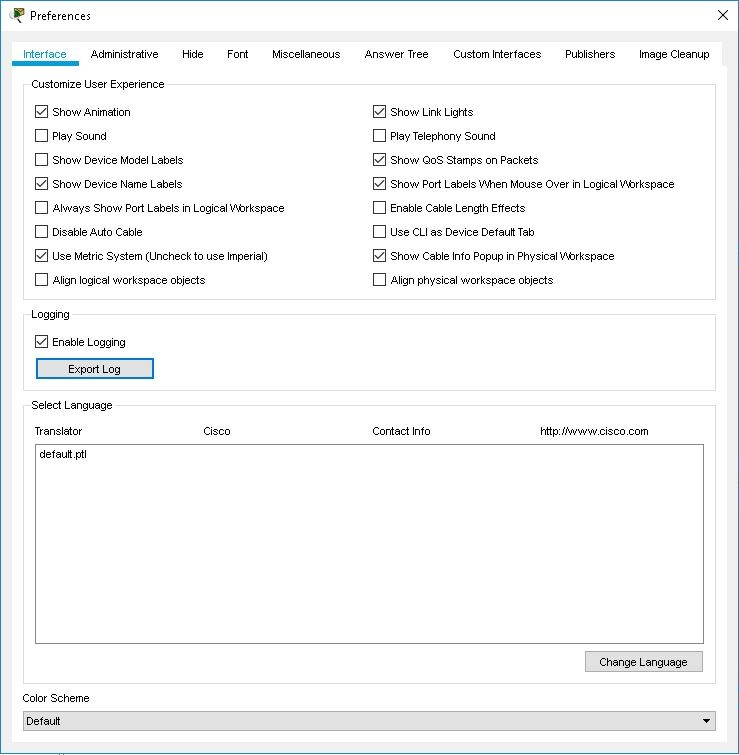
\includegraphics[width=0.55\linewidth]{img_9} 
        \linebreak
        \small {\bfseries Figura 5}: Ventana de configuración y seguimiento de comandos IOS.
    \end{center}

    \section{Cableado}
    Packet Tracer soporta una variada cantidad de conecciones de red, cada tipo de cable solo puede ser conectado a ciertas interfaces:
    \begin{center}
        \begin{tabular}{| p{5cm} | p{11cm} |}
            \hline
            {\bfseries TIPO DE CABLE} & {\bfseries DESCRIPCIÓN} \\\hline
            
\includegraphics[width=0.125\linewidth]{img_5} Consola & Las conexiones de tipo consola se pueden realizar entre computadoras, routers o switches. Se deben alcanzar ciertas condiciones para que una sesión de consola de una computadora funcione (las velocidades en ambos lados deben ser iguales, los bits de datos deben ser 7 para ambos u 8 para ambos, etc). \\\hline
            
\includegraphics[width=0.125\linewidth]{img_6} Cobre directo & Este tipo de cable es el estandar de conexiónentre dispositivos que operan en las diferentes capas del modelo OSI, por ejemplo hub a router, switch a pc, router a hub, etc. Se puede conectar a los puertos 10Mbps (ethernet), 100Mbps (Fast ethernet), 1000Mbps (Gigabit ethernet).\\\hline
            
\includegraphics[width=0.125\linewidth]{img_7} Cobre cruzado & Este cable es para conectar dispositivos que operan en la misma capa del modelo OSI (PC a PC, hub a hub, etc.) Se puede conectar a los puertos 10Mbps (ethernet), 100Mbps (Fast ethernet), 1000Mbps (Gigabit ethernet).\\\hline
            
\includegraphics[width=0.125\linewidth]{img_8} Fibra & Este cable se utiliza para conectar dispositivos que operen con puertos para fibra (100Mbps o 1000Mbps).\\\hline
        \end{tabular}
    \end{center} 

    \section{Interconexión cruzada de 2 computadoras}
    Para realizar la conexión entre 2 computadoras se selecciona del menú "End devices" (Ctrl+Alt+V) y se arrojan dos dispositivos PC en el espacio de trabajo lógico. A continuación en el menú "Conections" (Ctrl+Alt+O) se selecciona el cable correspondiente para este tipo de conexión, "Copper Cross-Over" (cobre cruzado), se hace un primer clic en la PC-0 seleccionando, en el menú desplegable que aparecerá, la opción FastEthernet0 (que hace referencia a la tarjeta de red disponible en esta PC) que será utilizada para conectar en la segunda computadora realizando el mismo paso.
    \begin{center}
        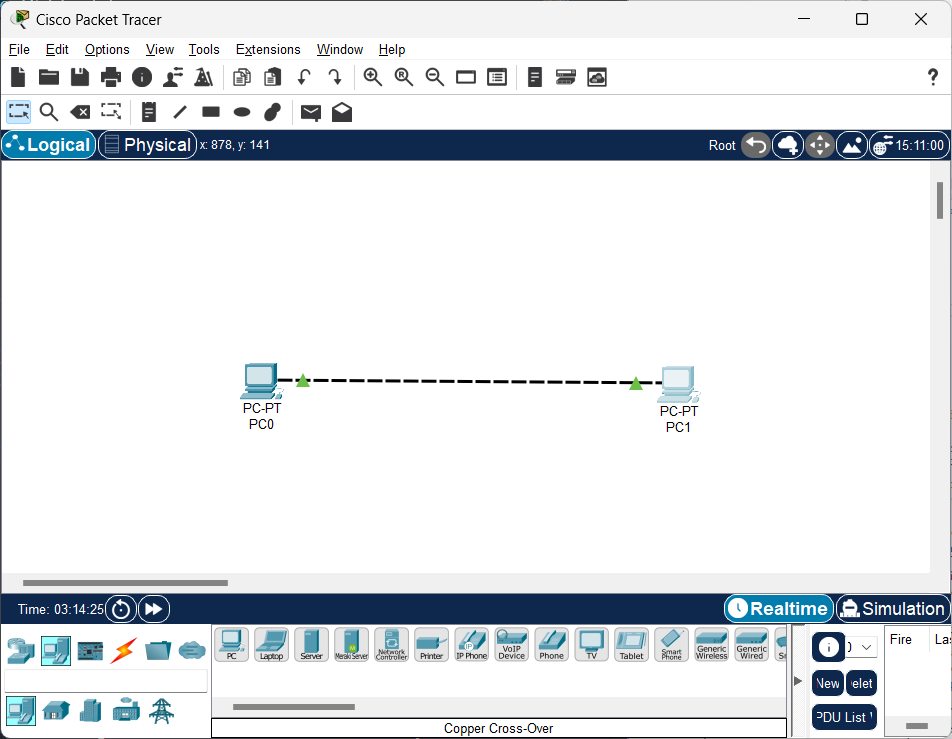
\includegraphics[width=0.65\linewidth]{img_10} 
        \linebreak
        \small {\bfseries Figura 6}: Conexión de 2 PC directo con cable cobre cruzado.
    \end{center}
    Una vez logrado esto, se debe configurar, en el menú {\bfseries Desktop - IP configuration} en cada computadora, la dirección IP, Máscara de Subred y Puerta de enlace predeterminada de manera que ambas computadoras compartan la misma puerta de enlace y tengan una numeración de IP diferente y contigua preferentemente (ya que no disponemos de un servidor con protocolo DHCP [Dinamyc Host Configuration Protocol])
    \begin{center}
        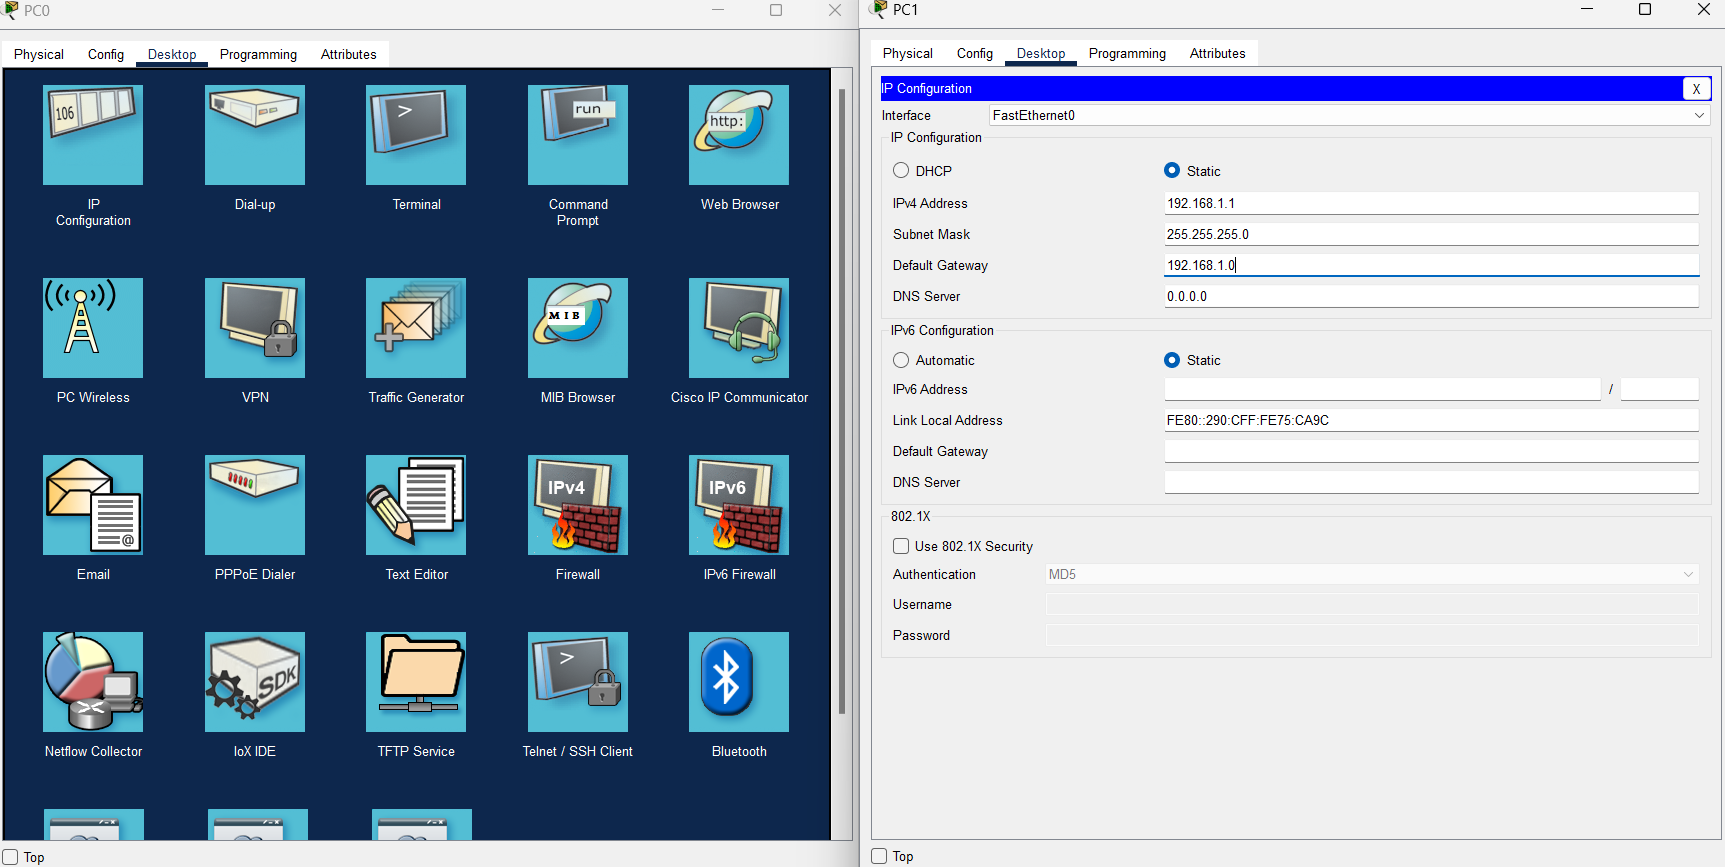
\includegraphics[width=0.9\linewidth]{img_12} 
        \linebreak
        \small {\bfseries Figura 7}: Conexión de 2 PC directo con cable cobre cruzado.
    \end{center}
    Por último realizar una comprobación básica realizando con el comando {\bfseries ping} en el "Command Promp" del escritorio de cada PC, que enviará 4 paquetes al destino indicado y nos informará si recibimos respuesta del mismo (tal como se muestra en la figura 8).
    \begin{center}
        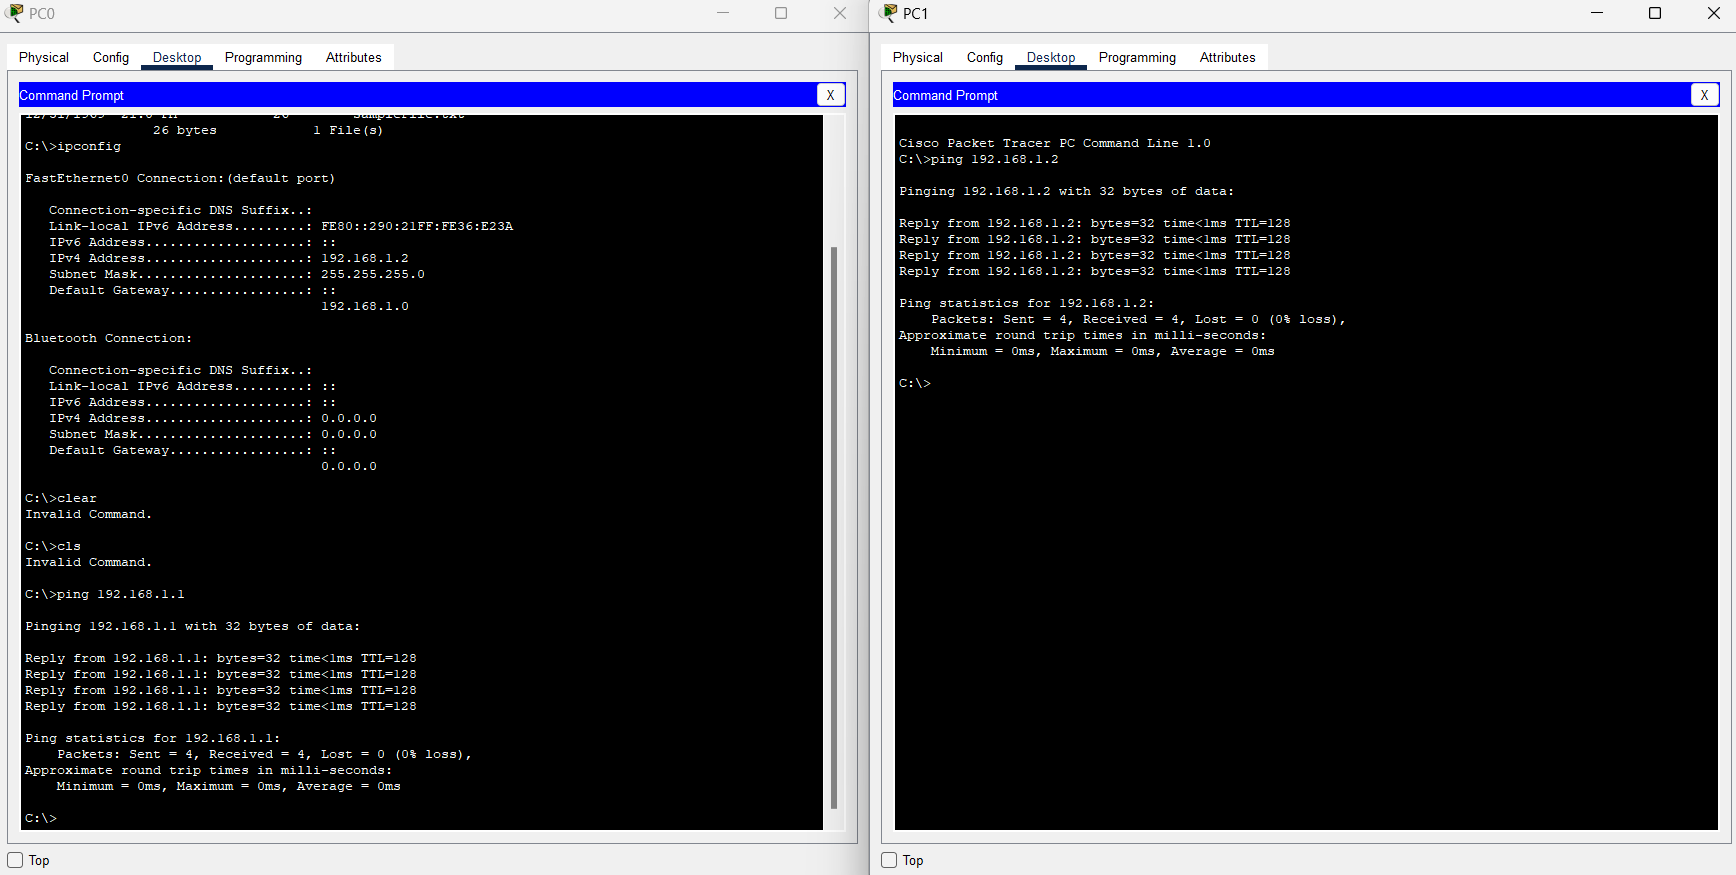
\includegraphics[width=0.9\linewidth]{img_11} 
        \linebreak
        \small {\bfseries Figura 8}: Comprobación de interconexión de dos computadoras con comando ping.
    \end{center}
    Si se envían y reciben correctamente los 4 paquetes, las computadoras se encuentran conectadas entre si.\linebreak
    Esta forma de conexión presenta la limitación de que solo se pueden conectar 2 máquinas entre si ya que cuentan con una única interfaz de conexión para el cable de cobre, y aún si tuvieran tarjetas de red adicionales no quedaría una configuración elegante.
    
    \pagebreak
    \section{Referencias}
        \begin{itemize}
            \item \href{https://github.com/MarianC312/Introduccion_Packet_Tracer}{Repositorio GitHub}
            \item \href{https://www.youtube.com/watch?v=qZB_biPOBwA}{CertBros - Cisco Packet Tracer - Everything you need to know.}
            \item \href{https://www.overleaf.com/learn}{Documentación Overleaf}
            \item \href{https://www.netacad.com/courses/packet-tracer}{Getting Started with Cisco Packet Tracer}
            \item \href{https://www.geeksforgeeks.org/how-to-configure-end-devices-on-packet-tracer/}{How to configure End Devices on Packet Tracer}
        \end{itemize}
\end{document}